\renewcommand{\thechapter}{\arabic{chapter}}
\setcounter{chapter}{7}

\chapter{Processus multimodal d'aide au diagnostic clinique}
\label{chap:chapter_8}
\chapterintro
Les travaux de la précédente partie ont porté sur le diagnostic de données malignes sur la modalité de \acrlong{mcr}, plus particulièrement de pathologies de \acrlong{lm} et de \acrlong{lmm}. Au premier niveau hiérarchique, soit celui des images, ces chapitres ont permis la mise en avant de méthodes de séparation des tissus sains, bénins et malins. Au second niveau hiérarchique, soit celui des lésions, ces méthodes permettent la prédiction des pathologies bénignes et malignes.\par

Ce nouveau chapitre rempli l'objectif de ce manuscrit en intégrant une dimension multimodale au processus de prise de décision. Tout d'abord, les aspects d'extraction de caractéristiques et de diagnostic par le biais de modèles de prédiction sont traités pour chacune des modalités présentes dans le jeu de données utilisé. De plus, la calibration de ces modèles de prédiction est envisagée afin de rendre cohérentes les décisions entre chacun d’entre eux. Puis, les processus multimodaux envisagés dans ce travail sont présentés selon deux axes~: une première méthode qualifiée comme sans mémoire, puis une seconde méthode qualifiée sous le terme d’avec mémoire. Finalement, les résultats obtenus à l'aide de ces méthodes sont présentés et discutés.\par
\newpage

\section{Méthodologie}
Lors de la \Cref{part:microscopy}, diverses méthodes de classification ont été proposées afin de gérer les données issues de la modalité de \gls{mcr} soit au niveau des images, soit au niveau des lésions. Outre le besoin de répondre à un certain nombre de verrous scientifiques, la réalisation de ces travaux est une une étape nécessaire de la mise en oeuvre du processus multimodal de ce manuscrit.\par

Néanmoins, à ce stade les méthodes proposées lors des précédents chapitres ne permettent que la prédiction au niveau de la modalité de \gls{mcr}. De plus, les méthodes de la littérature ne considèrent généralement que le diagnostic d'une modalité en particulier, sans considérer son intégration au sein d'un processus décisionnel plus global. Ces problématiques multimodales sont considérées dans de nombreux champs d'applications tels que l'identification d'individus~\cite{Lupu2008}, la conduite autonome~\cite{Xiao2019}, la reconnaissance vocale~\cite{Ngiam2011} ou encore du diagnostic de pathologies~\cite{Lim2014, Liu2015a}. Ces travaux concernent pour la plupart une prise de décision à partir de sources simultanées d'information, mais ne répondent pas à une problématique de prise de décision multimodale séquentielle.\par

Ainsi, ce dernier chapitre propose une méthodologie en plusieurs étapes pour permettre la mise en place d'un processus d'aide au diagnostic multimodal en milieu clinique. Ce chapitre ne se focalise pas sur la robustesse des diverses modalités, pour lesquelles d'une part sont reprises les propositions de la littérature propres aux modalités de photographie clinique et de dermatoscopie et d'autre part celle de ce manuscrit sur la \gls{mcr} formulés lors du \Cref{chap:chapter_7}. Par ailleurs, ce travail s'inspire pour certaines étapes, de travaux réalisés sur la fusion de données.

Pour parvenir à la réalisation de ce processus de décision multimodal, ce manuscrit propose de détailler les diverses étapes qui le composent, dont une représentation est fournie sur la \Cref{fig:scheme_multimodal_methodology}. Dans un premier temps, ce chapitre propose une mise au point sur les techniques permettant un diagnostic sur les modalités employées dans ce manuscrit. Dans un second temps, le principe de la calibration de modèle est présenté, dont l'utilisation est recommandée dans des contextes impliquant la collaboration de multiples modèles de prédiction. Dans un troisième temps, les processus multimodaux de prise de décision élaborés pour le besoin de cette problématique sont présentés, avec d'une part la considération d'un processus sans mémoire et d'autre part d'un processus avec mémoire. Pour finir, ce chapitre se termine par une présentation des résultats issus des méthodes proposées, suivi d'une discussion sur ceux-ci.\par

\begin{figure}[H]
    \centering
    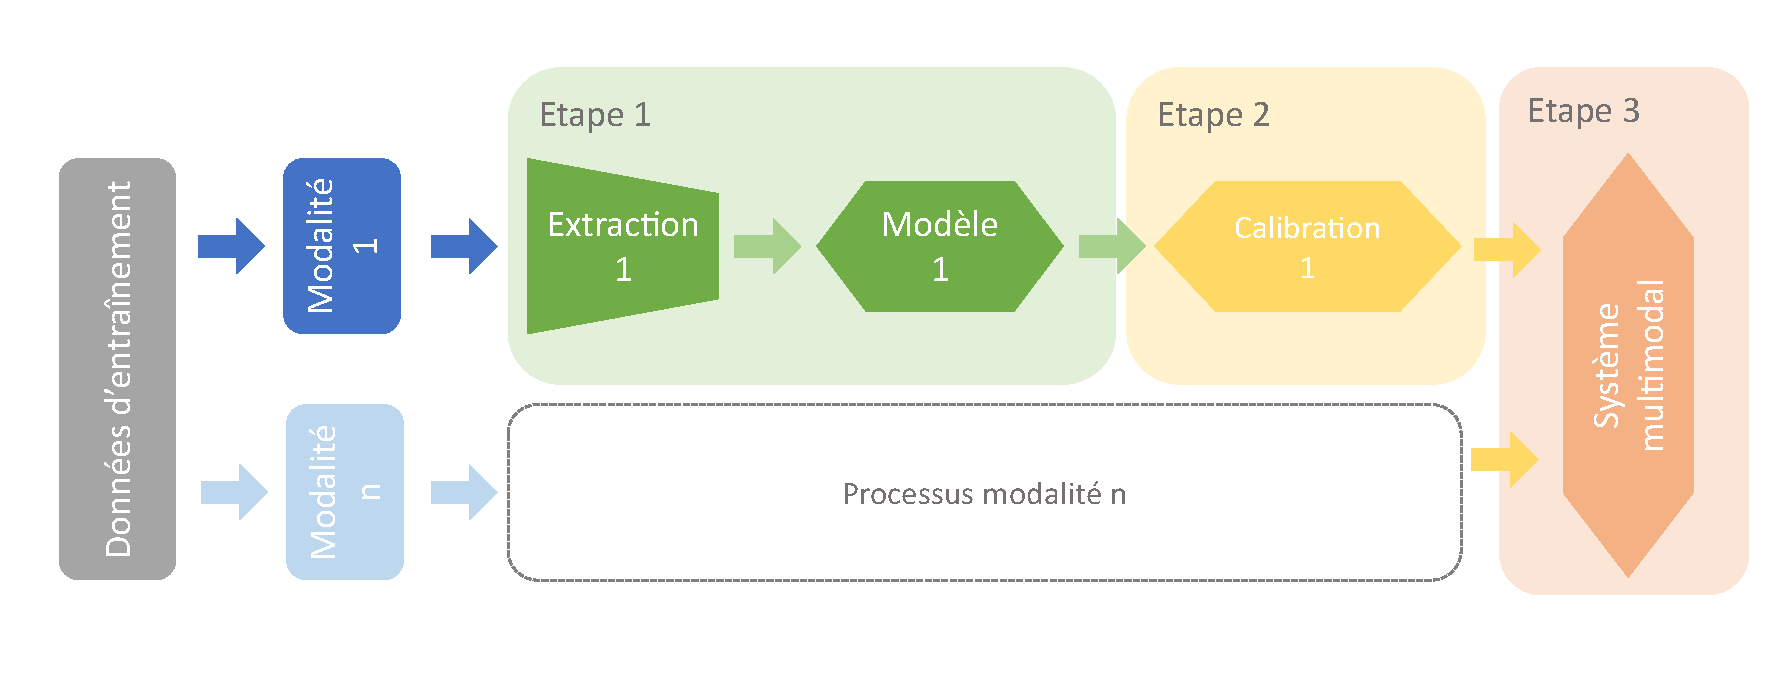
\includegraphics[width=0.9\linewidth]{contents/chapter_8/resources/scheme_multimodal_methodology.pdf}
    \caption{Schéma reprenant la progression de ce chapitre et l'interaction entre les différentes méthodes présentées.}
    \label{fig:scheme_multimodal_methodology}
\end{figure}\par

\section{Diagnostic des modalités}
\label{sec:modality_diagnosis}
Cette section se destine à la présentation des méthodes de diagnostic propres à chaque modalité. L'information brute n'étant pas utilisable en l'état, il est nécessaire de procéder à~:
\begin{inlinerate}
    \item sa réduction par l'extraction de caractéristiques pertinentes,
    \item la détection de données malignes à partir de cette information.
\end{inlinerate} La première sous-section décrit brièvement les méthodes employées tandis que la seconde sous-section apporte une pré-analyse de ces méthodes.\par

\subsection{Méthodes d'extraction et de détection}
Cette sous-section dédiée aux méthodes d'extraction et de détection des lésions débute par une brève étude des travaux menés sur la photographie clinique et sur la dermatoscopie. Ainsi, la plupart des travaux récents s'orientent autour de mécanismes d'apprentissage profond, dont certains travaux préconisent le recadrage des données employées~\cite{Li2018}. Dans ce travail, ce recadrage n'est réalisé que sur les données de photographie clinique jugées moins homogènes, que le reste des données mises à disposition. En termes de gestion de ces modalités d'imagerie, des travaux suggèrent l'utilisation d'architectures telles que Inception-V3~\cite{Esteva2017,Fan2020} ou encore ResNet-50~\cite{Xie2018, Alantari2018} associée à des couches de Global Pooling - Moyenne. Ces travaux orientés vers de la classification de lésions de la peau, procèdent à de l'extraction de caractéristiques ou à de la prédiction à partir de ces architectures. En ce qui concerne les méthodes d'extraction et de détection sur la modalité de \gls{mcr}, les méthodes de la \Cref{part:microscopy} sont mises à contribution dans ce chapitre. Ainsi, la méthode par transfert de connaissances par utilisation de l'architecture ResNet-50 entraîné sur ImageNet et couplé à une couche de Globale Pooling - Moyenne permet les meilleurs résultats dans ces conditions. Afin d'uniformiser l'extraction de caractéristiques de ces diverses modalités et par contraintes matérielles, le transfert de connaissance est préféré pour permettre l'extraction de caractéristiques, avec pour choix d'architecture ResNet-50.\par

D'une part, pour permettre une prédiction sur les données de photographie clinique et de dermatoscopie, ce travail privilégie l'utilisation d'un modèle \gls{svm} à noyau linéaire à la fois stable et robuste dans la plupart des situations. Ces modalités ne mettant à disposition qu’une unique image, ces deux modalités mettent à disposition un vecteur de taille 1 $\pm$ 2048. D'autre part, pour permettre une prédiction sur les données de \gls{mcr} ce travail reprend les méthodes de prédiction de la \Cref{part:microscopy}, et notamment l'utilisation d'un modèle par instance multiple de type \gls{nsk} considéré comme le plus performant dans un contexte ou le nombre de données est variable. En addition, afin de conserver une dimension de vecteur de caractéristique régulière pour certains besoins à venir, ce travail a eu recours aux méthodes de type moyenne, maximum ou de norme $p$ avec des valeurs arbitraires de 4, 6 et 8 comme suggéré par certains travaux de la littérature~\cite{Li2016,Xu2017}.\par

Les hyperparamètres associés au modèles de prédiction cités sont listés dans la \Cref{tab:multimodal_models_parameters}. Par ailleurs, le modèles \gls{svm} employés par ce travail provient de la bibliothèque logicielle \textit{Scikit-learn}~\cite{pedregosa2011}, tandis que l'implémentation de modèles \gls{nsk} utilise la librairie logicielle \textit{MISVM}~\cite{Doran2014}.\par
\begin{table}[H]
    \centering
    \begin{tabular}{lll}
    \toprule
    \textbf{Méthode}    & \textbf{Paramètre}& \textbf{Valeurs}                                  \\ \midrule
    \gls{svm}           & \multirow{2}{*}{C}& \multirow{2}{*}{[0,01, 0,1, 1, 10, 100, 1000]}    \\ \cline{1-1}
    \gls{nsk}           &                   &                                                   \\ \bottomrule 
    \end{tabular}    
    \caption{Table reprenant les divers modèles utilisant le principe d'\gls{mil} pour réaliser une classification au niveau lésionnel, ainsi que leurs hyperparamètres associés.}
    \label{tab:multimodal_models_parameters}
\end{table}\par
\clearpage

\subsection{Pré-analyse}
Cette pré-analyse des méthodes de classification permet d'obtenir une vision des performances obtenues à chaque modalité. Pour cela, les évaluations ci-dessous sont réalisées à l'aide d'une valeur de validation croisée de $k$ égale à 10, comme utilisé dans les prochaines expérimentations de ce chapitre et dont les termes sont décrits plus en détail dans la section résultats.\par

Ainsi, la \Cref{tab:results_multimodality_modalities} permet de mettre en avant une capacité de discrimination des deux classes croissantes pour les diverses modalités sollicitées dans cette étude. Par cette méthode de prise en charge, un \fscore{} pondéré entre les classes bénigne et maligne de 0,62 associé à un écart-type de 0,08 est obtenu sur la photographie clinique, de 0,74 associé à un écart-type de 0,11 sur la dermatoscopie et de 0,80 associé à un écart-type de 0,12 sur la \gls{mcr} ; un \fscore{} sur la classe maligne de 0,68 associé à un écart-type de 0,09 est obtenu sur la photographie clinique, de 0,79 associé à un écart-type de 0,09 sur la dermatoscopie et de 0,84 associé à un écart-type de 0,11 sur la \gls{mcr}. Cette pertinence croissante du diagnostic est exploitée au sein des processus multimodaux proposés dans les prochaines sections.\par

\begin{table}[H]
    \centering
    \begin{tabular}{llccc} \toprule
        \multicolumn{1}{l}{}     & Modalité      & Précision    & Rappel        & \Fscore{}     \\ \midrule
        \multirow{3}{*}{Pondéré} & Photographie  & 0,63 $\pm$ 0,08& 0,62 $\pm$ 0,07 & 0,62 $\pm$ 0,08 \\
                                 & Dermatoscopie & 0,74 $\pm$ 0,11& 0,74 $\pm$ 0,10 & 0,74 $\pm$ 0,11 \\
                                 & Microscopie   & 0,80 $\pm$ 0,11& 0,80 $\pm$ 0,12 & 0,80 $\pm$ 0,12 \\ \midrule
        \multirow{3}{*}{Malin}   & Photographie  & 0,71 $\pm$ 0,12& 0,66 $\pm$ 0,09 & 0,68 $\pm$ 0,09 \\
                                 & Dermatoscopie & 0,79 $\pm$ 0,13& 0,79 $\pm$ 0,12 & 0,79 $\pm$ 0,09 \\
                                 & Microscopie   & 0,85 $\pm$ 0,11& 0,83 $\pm$ 0,12 & 0,84 $\pm$ 0,11 \\ \bottomrule
    \end{tabular}
    \caption{Pré-résultats obtenus à partir des méthodes de classification employées sur chacune des modalités utilisées dans ce processus.}
    \label{tab:results_multimodality_modalities}
\end{table}

Enfin, la \Cref{tab:results_multimodality_weighted_microscopy} permet de mesurer l'efficacité des méthodes de réduction employées \textbf{par l'utilisation d'un modèle \gls{svm} à noyau linéaire}. Cette table met en évidence les résultats par pondération sur les deux classes, la méthode de réduction par la moyenne est à la fois plus performante et plus stable que les autres méthodes avec un \fscore{} de 0,84 associé à un écart-type de 0,07. Dans la suite des travaux nécessitant l'utilisation des caractéristiques issues de la modalité de \gls{mcr}, cette \textbf{méthode de réduction par la moyenne} est privilégiée afin d'obtenir un vecteur de caractéristiques constant.\par

\begin{table}[H]
    \centering
    \begin{tabular}{lccc} \toprule
        Réduction           & Précision             & Rappel                & \Fscore{}             \\ \midrule
        \textbf{Moyenne}    & \textbf{0,84 $\pm$ 0,07}& \textbf{0,83 $\pm$ 0,07}& \textbf{0,84 $\pm$ 0,07}\\
        Maximum             & 0,83 $\pm$ 0,12         & 0,83 $\pm$ 0,12         & 0,83 $\pm$ 0,12         \\
        Norme $p$ - 4       & 0,82 $\pm$ 0,12         & 0,82 $\pm$ 0,12         & 0,82 $\pm$ 0,12         \\
        Norme $p$ - 6       & 0,83 $\pm$ 0,12         & 0,83 $\pm$ 0,13         & 0,83 $\pm$ 0,13         \\
        Norme $p$ - 8       & 0,83 $\pm$ 0,12         & 0,83 $\pm$ 0,12         & 0,83 $\pm$ 0,12         \\ \bottomrule
    \end{tabular}
    \caption{Pré-résultats pondérés sur la classe bénigne et maligne, permettant de mesurer l'efficacité des méthodes de réduction des caractéristiques par classification à l'aide d'un modèle \gls{svm}.}
    \label{tab:results_multimodality_weighted_microscopy}
\end{table}

\clearpage

\section{Calibration de modèles}
\label{sec:calibrate_models}
La majeure partie des modèles de classification mettent à disposition des scores représentant l'appartenance à chacune des classes de la problématique visée. Ces scores sont à l'origine des prédictions de ces modèles et peuvent être obtenus de manière complémentaire à la prédiction. Ainsi, la décision résultante n'est bien souvent que la manifestation de la classe ayant achevé le score de prédiction le plus élevé.\par

Malheureusement, ces scores n'ont de sens que dans le contexte dans lequel ils ont été obtenus et ne conviennent pas lorsque plusieurs sources d'information différentes sont combinées. Ainsi, une estimation précise de la \textbf{probabilité} d'appartenance à chacune des classes est un indicateur plus pertinent dans ce type de situation, ayant un sens en dehors du champ d'action propre à chacun de ces modèles~\cite{Zadrozny2002}.\par

Diverses méthodes sont proposées afin de transformer ces scores en probabilités, tout d'abord sur des problématiques binaires, puis plus tardivement sur des problématiques à classes multiples. Ce principe de transformation des scores en probabilités porte le nom de processus de \textbf{calibration}, et cherche à faire converger $P(c|s(x)=s)$ vers $s(x)=s$~\cite{Zadrozny2002}. Ces méthodes proposent de corriger ces scores à l'aide de \textit{fonctions de transfert} de différentes formes, dont les performances peuvent être appréhendées à l'aide du \textbf{score de Brier}. Ce score dont la formulation est exprimée sur l'\Cref{eq:brier_score} avec $p_i$ la probabilité d'un événement et $o_i$ son observation réelle, s'accompagne de faibles valeurs lorsque la calibration du modèle est supposé parfaite. De plus, la calibration d'un modèle peut être visualisée de manière binaire à l'aide de \textbf{courbes de fiabilité}, représentées à l'aide de lots de données constitués de scores semblables, et dont le taux réel d'éléments positifs propre à un lot est exprimé selon les scores moyen de prédiction de celui-ci.\par

\begin{equation} 
    \label{eq:brier_score}
    Brier = \frac{1}{N}\sum\limits _{i=1}^{N}(p_i-o_i)^2 
\end{equation}

Ainsi, la littérature propose diverses méthodes pour permettre de rectifier ces scores, dont les calibrations~:
\begin{inlinerate}
    \item \textit{Logistique}~\cite{Friedman2000},
    \item \textit{Sigmoïde}~\cite{Platt2000,kull2017b},
    \item \textit{Isotonique}~\cite{Zadrozny2002},
    \item \textit{Bayésienne en Quantiles}~\cite{Naeini2015},
    \item ou encore \textit{Bêta}~\cite{Kull2017}.
\end{inlinerate} Dans la mesure où ce chapitre répond à une problématique binaire, seules les méthodes de calibration binaire sont considérées, dont les méthodes \textbf{sigmoïde} et \textbf{isotonique} sont les majeurs représentants. Ainsi, \textbf{la calibration sigmoïde} se base sur l'hypothèse que les scores issues d'un modèle de prédiction vont suivre une courbe de type \textit{sigmoïde}, et consiste à approcher par une même fonction ces scores afin de les rectifier~\cite{Niculescu2005}. Cette fonction est représentée sur l'\Cref{eq:sigmoid_calibration}, dont les deux paramètres de forme $A$ et $B$ sont recherchés par optimisation. À l'instar de la calibration sigmoïde, \textbf{la calibration isotonique} est une forme plus généralisée permettant d'approcher une plus grande multitude de tendances, dont l'unique condition requiert d'être \textit{isotonique} ou monotone croissante~\cite{Niculescu2005}. Les processus de calibration nécessitent l'utilisation de deux ensemble de données séparés et dédiés à l'entrainement et à la validation. La mise en œuvre de ces calibrations se base sur la librairie logicielle \textit{Scikit-learn}~\cite{pedregosa2011}.\par

\begin{equation}
    \mathrm{P}(y=1 \mid x)=\frac{1}{1+\exp (A f(x)+B)}
    \label{eq:sigmoid_calibration}
\end{equation}

% Ces modes de calibration sont recensés dans la \Cref{tab:multimodal_calibration_values} et leurs mise en œuvre se base sur la librairie logicielle \textit{Scikit-learn}~\cite{pedregosa2011}. 
% \begin{table}[H]
%     \centering
%     \begin{tabular}{ll}
%         \toprule 
%         Paramètre                   & Valeurs                       \\ \midrule
%         Mode de calibration         & [Sans, Isotonique, Sigmoïde]  \\ \bottomrule
%     \end{tabular}
%     \caption{Table de recensement des divers modes de calibration proposés pour le processus multimodal.}
%     \label{tab:multimodal_calibration_values}
% \end{table}
\clearpage

\section{Processus d'aide au diagnostic multimodal}
Cette section se consacre à la mise en place d'un processus d'aide au diagnostic multimodal. Son objectif est de donner une consistance à l'information provenant des diverses modalités d'images, en optimisant le nombre d'individus traités à chacune d'entre elles tout en conservant une performance de détection maximale. D'une part dans une première sous-section, ce processus est traité sous deux aspects différents dans le but de résoudre cette problématique. D'autre part, une présentation du modèle permettant la détermination des seuil clés est réalisée.

\subsection{Présentation des processus}
Les processus multimodaux envisagé pour la résolution de la problématique s'inspirent de la procédure actuelle réalisée par les dermatologues. Dans ce processus clinique type, une lésion est prise en charge à partir de modalités simples d'accès à des modalités plus difficile d'accès. Concrètement, le processus type sollicite respectivement la photographie clinique, la dermatoscopie et la microscopie confocale. Le dermatologue va recourir à une modalité supplémentaire en cas de doute lors du diagnostic, caractérisé dans ce travail par \textbf{la zone grise}. Ce travail propose de reproduire ce comportement à l'aide d'une démarche algorithmique, en sollicitant les modalités respectivement dans l'ordre précédent. Ainsi, deux types d'approches sont développés lors des prochains paragraphes, exploitant ce principe de processus \textbf{séquentiel} et de \textit{zone grise}.\par

D'une part, le \textbf{processus sans mémoire} consiste à mobiliser les modalités \textit{indépendamment} les unes des autres. Ce type de processus correspond à la prise en charge médicale d'un patient sans communication d'information entre les divers examens menés. Dans un premier temps, l'étape d'entraînement consiste à traiter indépendamment chaque modalité, \textbf{sur une fraction des données arbitrairement consacrée à cette étape}, dans le but d'obtenir un modèle de prédiction optimal selon les termes de la \Cref{sec:modality_diagnosis}. Par ailleurs, c'est également à ce stade de l'entraînement que la méthode de calibration est réalisée selon les termes énoncés lors de la \Cref{sec:calibrate_models}. Dans un second temps, cette même étape d'entraînement consiste à déterminer des seuils de confiance, \textbf{sur les données mise à disposition restantes}, permettant de délimiter la zone grise à chaque étape du processus, dont le fonctionnement est détaillé en \Cref{sec:multimodal_confidence_model}. La \Cref{fig:scheme_multimodal_process_without} représente ce concept sous forme de schéma.\par

D'autre part, le \textbf{processus avec mémoire} consiste à mobiliser les modalités en \textit{conservant l'information} recueillie à l'aide des précédentes modalités. Ce type de processus peut être mis en parallèle avec celui d'un praticien qui réalise l'ensemble des examens, ou avec la constitution d'un dossier patient. Dans un premier temps, l'étape consiste à construire des modèles de prédiction cumulatifs \textbf{sur une fraction des données, attribués à l'entraînement}, par agrégation des caractéristiques extraites dont le principe à été adopté dans des travaux de biométrie~\cite{Krishneswari2012}. À nouveau, il est possible de procéder à la calibration des modèles à ce stade du processus. Dans un second temps, ce processus procède également à la détermination des seuils de confiance, \textbf{sur les données mises à disposition restantes}, permettant de délimiter la zone grise à chaque étape du processus et dont le principe de fonctionnement est détaillé en \Cref{sec:multimodal_confidence_model}. Ce processus est représenté sous forme de schéma à l'aide de la \Cref{fig:scheme_multimodal_process_with}.\par

\begin{landscape}
\begin{figure}[H]
    \centering
    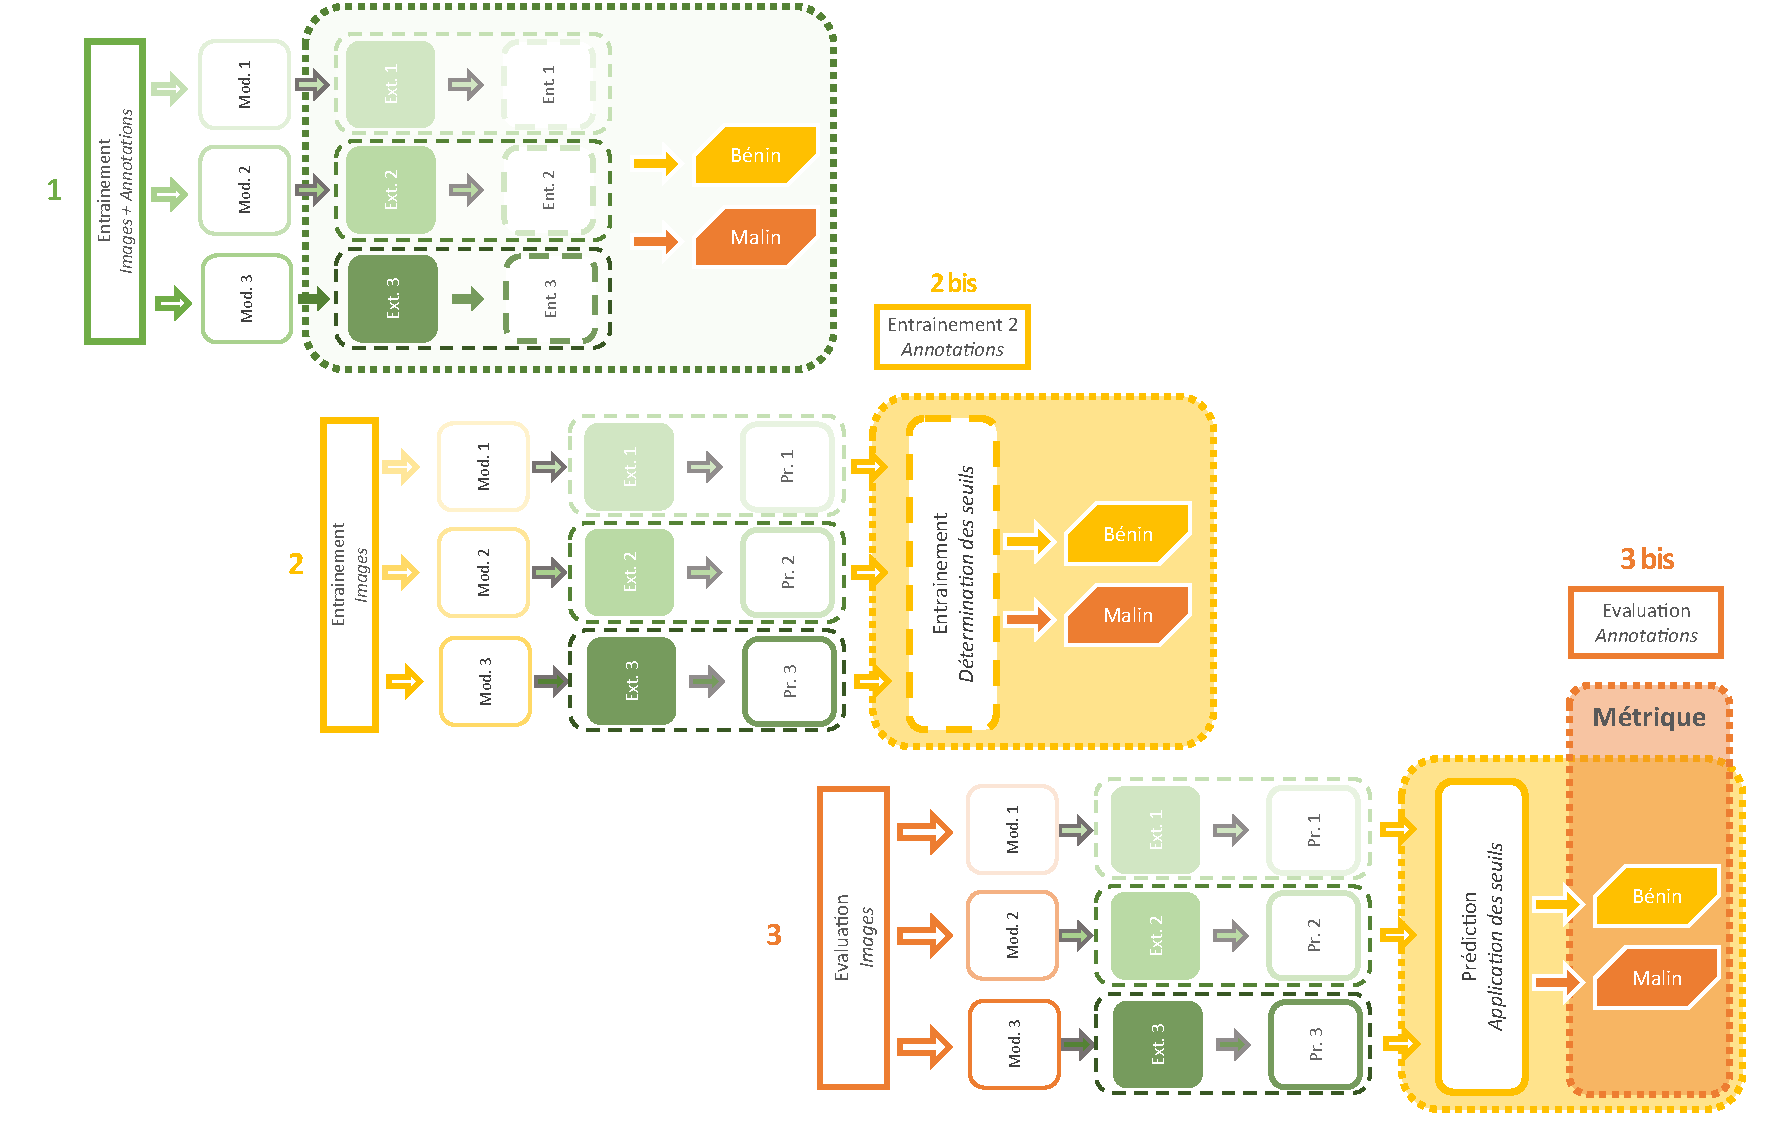
\includegraphics[width=0.85\linewidth]{contents/chapter_8/resources/scheme_multimodal_process_without.pdf}
    \caption{Schéma de fonctionnement du processus multimodal sans mémoire, dont la phase d'entraînement est réalisée en deux temps. Dans un premier temps, un entraînement est réalisé sur les modèles de prédiction au niveau de chaque modalité mise à disposition par le premier jeu de données d'entraînement. Dans un second temps, le modèle de gestion optimise les seuils de confiance à l'aide du second jeu de données d'entraînement. L'entraînement achevé, les performances sont mesurées sur les données d'évaluation.}
    \label{fig:scheme_multimodal_process_without}
\end{figure}\par
\end{landscape}

\begin{landscape}
\begin{figure}[H]
    \centering
    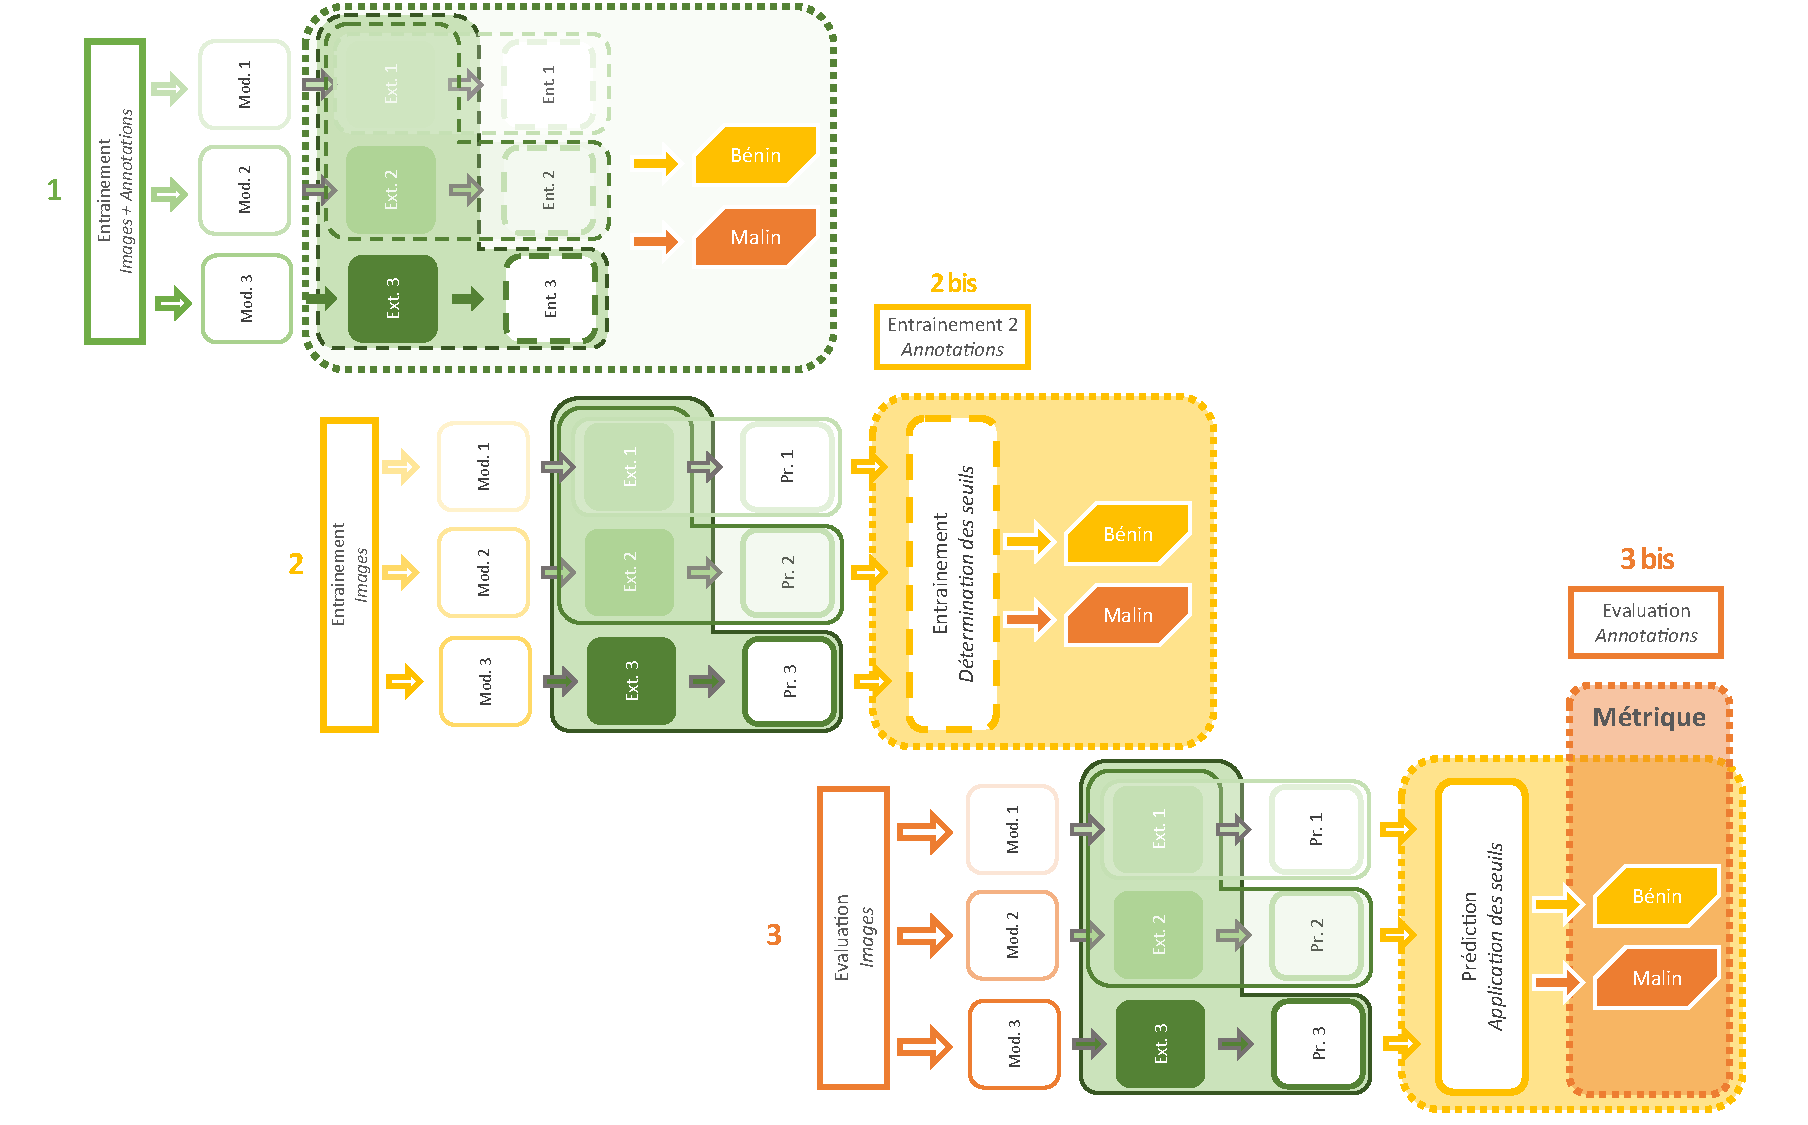
\includegraphics[width=0.85\linewidth]{contents/chapter_8/resources/scheme_multimodal_process_with.pdf}
    \caption{Schéma de fonctionnement du processus multimodal avec mémoire, dont la phase d'entraînement est réalisée en deux temps. Dans un premier temps, un entraînement est réalisé sur les modèles de prédiction propre à chaque étape du processus clinique et pour lesquels les données précédemment acquises sont cumulées. Dans un second temps, le modèle de gestion optimise les seuils de confiance à l'aide du second jeu de données d'entraînement. L'entraînement achevé, les performances sont mesurées sur les données d'évaluation.}
    \label{fig:scheme_multimodal_process_with}
\end{figure}\par
\end{landscape}

\subsection{Modèle d'optimisation des seuils de confiance}
\label{sec:multimodal_confidence_model}
Lors de la précédente sous-section ont été envisagés divers modes de prise en charge multimodal. Néanmoins, ces deux processus en l'état ne permettent pas leur utilisation. Cette seconde sous-section consacrée aux processus par modalités multiples clôture cet aspect par l'apport de méthodes permettant de déterminer des seuils de confiances permettant la prise en charge de modalité en modalité.\par

L'entrée nécessaire à l'entraînement de ce modèle se constitue d'un \textbf{couple $x$ et $y$}. Ce couple se constitue d'une part de \textbf{$x$ une matrice de scores de taille $n \times m \times c$}, avec $n$ correspondant au nombre d'échantillons, avec $m$ correspond au nombre de modalités et avec $c$ le nombre de classes. D'autre part, ce couple se constitue de \textbf{$y$ une matrice de sorties attendues de taille $n \times 1$}, avec $n$ le nombre d'échantillons. Bien que le but recherché soit l'optimisation de la prise en charge des lésions, celui-ci s'inscrit dans une démarche clinique. Ainsi, \textbf{une emphase particulière est consacrée à la maximisation d'une métrique}, par défaut le \fscore{} bien que celui-ci puisse être substitué par d'autres métriques.\par

Pour effectuer cette tâche, une première hypothèse dans laquelle l'on considère qu'un \textbf{unique} seuil de confiance est suffisant pour délimiter la zone grise d'une modalité isolément de son appartenance à une classe et, une seconde hypothèse dans laquelle l'on considère que de \textbf{multiples} seuils de confiance relatifs à leurs classes respectives sont nécessaires. Ce concept est schématisé sur la \Cref{fig:scheme_multimodal_treshold}.\par

\begin{figure}[H]
    \centering
    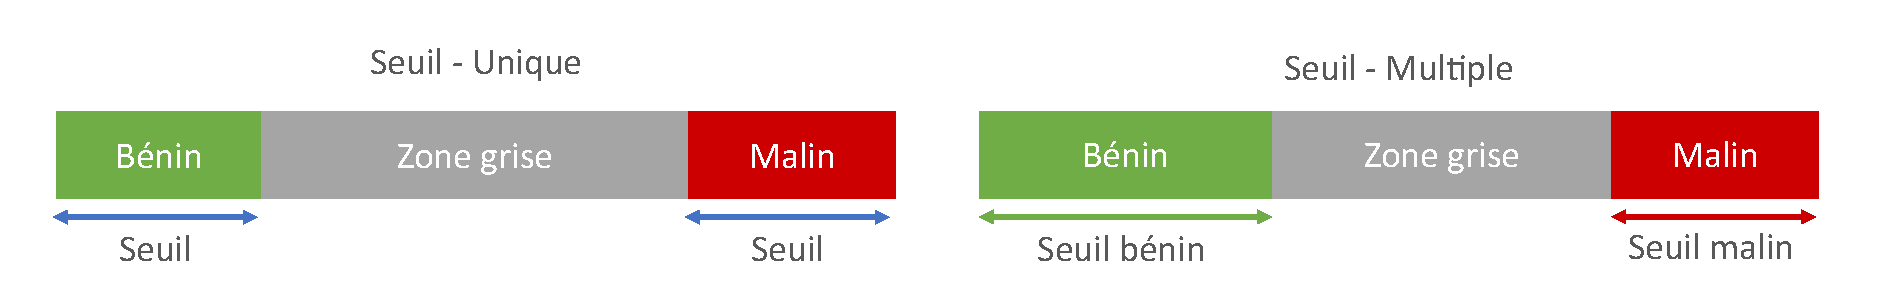
\includegraphics[width=\linewidth]{contents/chapter_8/resources/scheme_multimodal_treshold.pdf}
    \caption{Schéma de représentation des concepts de seuil unique et multiple.}
    \label{fig:scheme_multimodal_treshold}
\end{figure}\par

Au \textbf{niveau des modalités}, l'identification de ces seuils peut être réalisée soit de manière \textbf{croissante} à partir de la modalité la moins précise en \textit{améliorant} la métrique vers un score idéal, soit de manière \textbf{décroissante} à partant de la modalité la plus précise en \textit{dégradant} la métrique jugée idéale. Au \textbf{niveau de la détection} au sein d'une modalité, l'identification de ces seuils peut être réalisée soit de manière \textbf{croissante} en \textit{augmentant} la valeur des seuils jusqu'à détecter une baisse de la métrique, soit de manière \textbf{décroissante} en \textit{réduisant} la valeur des seuils jusqu'à détecter une baisse de la métrique. Ces divers paramètres sont évalués et sont synthétisés dans la \Cref{tab:multimodal_confidence_model_values}.\par

\begin{table}[H]
    \centering
    \begin{tabular}{ll}
        \toprule 
        Paramètre                   & Valeurs                   \\ \midrule
        Seuil                       & [Unique, Multiple]        \\ \midrule
        Modalités                   & [Croissante, Décroissante]\\ \midrule
        Détection                   & [Croissante, Décroissante]\\ \bottomrule
    \end{tabular}
    \caption{Table de recensement des divers paramètres évalués pour la détermination des seuils de confiance optimaux au sein du processus multimodal.}
    \label{tab:multimodal_confidence_model_values}
\end{table}
 
\clearpage

\section{Présentation des résultats}
Cette section se destine à la présentation des résultats issus des méthodes précédemment énoncées. Dans un premier temps, cette section procède à la présentation du protocole d'expérimentation, comprenant le processus de validation et métrique associé ainsi que l'organisation des résultats. Puis dans un second temps, les divers résultats issus des expériences mentionnées précédemment sont développés.\par

\subsection{Protocole d’expérimentation}
Les divers résultats d'évaluations présentés par la suite sont obtenus par l'utilisation d'une \textbf{validation croisée imbriquée} dont le principe favorise l'obtention de métriques plus objectives sur les performances du système évalué~\cite{Cawley2010}. De plus, cette structure de validation est démontrée empiriquement moins sensible au biais et à la variance lorsque celle-ci est couplée à des valeurs de $k$ comprises entre 5 et 10 pour l'évaluation~\cite{James2000}. Lors du précédent chapitre, une valeur de $k$ égale à 10 avait été choisie dû à la faible diversité de combinaisons de méthodes proposée. De manière similaire, ce chapitre opte également \textbf{pour une valeur de $k$ égale à 10 pour la boucle d'évaluation} pour ces mêmes raisons. Une \textbf{valeur de $k$ égale à 2 est utilisée pour la boucle de validation}, jugée suffisante afin de déterminer la meilleure combinaison d'hyperparamètres.\par

En termes d'apprentissage, l'entraînement des modèles de prédiction au niveau des modalités est jugé plus coûteux que l'entraînement nécessaire à la définition des seuils de confiance sur les modèles proposés. Ainsi, sur les 9 lots mis à disposition du processus d'entraînement, \textbf{8 lots sont attribués à l'étape d'entraînement des modalités} tandis que \textbf{le dernier lot est attribué au modèle d"optimisation des seuils de confiance}.\par

Afin de régler au mieux les modèles présentés dans ce chapitre et de donner une évaluation objective malgré les déséquilibres d'annotations, le choix se porte sur le \textbf{\fscore{}}. Cette métrique permet une représentation conjointe des mesures de précision et de rappel au sein d'une même métrique binaire. Dans un premier temps, une valeur pondérée de ce \fscore{} selon les classes bénignes et malignes est recensée lors de la présentation des résultats pour chacune des expérimentations. Dans un second temps, la valeur de ce \fscore{} selon la classe maligne est relevée pour les systèmes jugés les plus pertinents. Conjointement, les valeurs de \textbf{sensibilité} et de \textbf{spécificité} sont renseignées de manière complémentaire au \fscore{} afin d'obtenir une vision plus complète des performances réelles de ces systèmes. Ces valeurs permettent une mise en parallèle avec les mesures de l'article de Cinotti et al.~\cite{Cinotti2016}.\par

Dans un premier temps, ce travail propose de présenter les résultats des expérimentations menées \textbf{sur le processus séquentiel sans mémoire} puis \textbf{sur le processus séquentiel avec mémoire}. Les résultats pondérés sont présentés pour l'ensemble des données et des expériences de ces deux types de processus. Ensuite, les résultats sont focalisés sur les expériences jugées les plus fonctionnelles de ce manuscrit et présentent les résultats détaillés sur la classe maligne, d'une part sur l'ensemble des lésions cliniques du jeu de données et d'autres part sur les pathologies de \gls{lm} et \gls{lmm}.\par

Dans un second temps, les données associées aux tables de résultats sont mises à disposition de manière complémentaire. Ainsi, les données de calibration des processus retenus sont mises à disposition du lecteur, pour permettre une meilleure compréhension de ces derniers. Pour finir, les résultats de simulation de prise en charge des lésions sont présentés avant de finir cette section.\par
\clearpage

\subsection{Résultats des expérimentation}
Cette section débute par la présentation des résultats du \textbf{processus multimodal sans mémoire}. Sans calibration, un \fscore{} de 0,80 associé à un écart-type de 0,10 est obtenu par \textbf{la méthode à seuil unique par modalités décroissantes et détection croissante}. À l'aide de la calibration isotonique, un \fscore{} de 0,71 associé à un écart-type de 0,16 est obtenu par \textbf{la méthode à seuils multiples par modalités décroissantes et détection croissante}. Enfin, à l'aide de la calibration sigmoïde, un \fscore{} de 0,79 associé à un écart-type de 0,10 sont obtenus par \textbf{des méthodes à seuil unique par modalités décroissantes et détection croissante / décroissante}. Les résultats de ce premier processus peuvent être visualisés dans la \Cref{tab:results_multimodal_process_without}.\par

\begin{table}[H]
    \centering
    \begin{tabular}{lllccc}
        \toprule 
        Seuil                       & Modalités                         & Détection         & Sans                          & Isotonique            & Sigmoïde                      \\ \midrule
        \multirow{4}{*}{Unique}     & \multirow{2}{*}{Croissante}       & Croissante        & 0,72 $\pm$ 0,14                 & 0,65 $\pm$ 0,14         & 0,66 $\pm$ 0,10                 \\ \cline{3-6}
                                    &                                   & Décroissante      & 0,72 $\pm$ 0,14                 & 0,64 $\pm$ 0,12         & 0,65 $\pm$ 0,09                 \\ \cline{2-6}
                                    & \multirow{2}{*}{Décroissante}     & \hcell Croissante & \hcell \textbf{0,80 $\pm$ 0,10} & \hcell 0,61 $\pm$ 0,11  & \hcell \textbf{0,79 $\pm$ 0,10} \\ \cline{3-6}
                                    &                                   & Décroissante      & 0,80 $\pm$ 0,11                 & 0,60 $\pm$ 0,13         & \textbf{0,79 $\pm$ 0,10}        \\ \cline{1-6}
        \multirow{4}{*}{Multiple}   & \multirow{2}{*}{Croissante}       & Croissante        & 0,71 $\pm$ 0,09                 & 0,64 $\pm$ 0,18         & 0,71 $\pm$ 0,13                 \\ \cline{3-6}
                                    &                                   & Décroissante      & 0,71 $\pm$ 0,09                 & 0,63 $\pm$ 0,17         & 0,70 $\pm$ 0,14                 \\ \cline{2-6}
                                    & \multirow{2}{*}{Décroissante}     & Croissante        & 0,77 $\pm$ 0,13                 & \textbf{0,71 $\pm$ 0,16}& 0,77 $\pm$ 0,12                 \\ \cline{3-6}
                                    &                                   & Décroissante      & 0,77 $\pm$ 0,13                 & 0,68 $\pm$ 0,14         & 0,77 $\pm$ 0,12                 \\ \bottomrule
    \end{tabular}
    \caption{Table de résultats issus de l'application du processus multimodal sans mémoire. Ces résultats sont exprimés à l'aide du \fscore{} et sont issus d'une prise en charge de l'ensemble des cas cliniques mis à disposition de ce manuscrit.}
    \label{tab:results_multimodal_process_without}
\end{table}

Ce second paragraphe procède à la présentation des résultats du \textbf{processus multimodal avec mémoire}. Sans calibration, un \fscore{} de 0,82 associé à un écart-type de 0,08 est obtenu par \textbf{la méthode à seuils multiples par modalités décroissantes et détection croissante}. À l'aide de la calibration isotonique, un \fscore{} de 0,82 associé à un écart-type de 0,10 sont obtenus d'une part par \textbf{la méthode à seuil unique par modalités décroissantes et détection croissante} et d'autre part par \textbf{la méthode à seuils multiples par modalités décroissantes et détection croissante}. Enfin, à l'aide d'une calibration sigmoïde, un \fscore{} de 0,82 associé à un écart-type de 0,11 est obtenu par \textbf{la méthode à seuil unique par modalités décroissantes et détection croissante}. Les résultats liés à ce second processus peuvent être visualisés dans la \Cref{tab:results_multimodal_process_with}.\par

\begin{table}[H]
    \centering
    \begin{tabular}{lllccc}
        \toprule 
        Seuil                       & Modalités                         & Détection         & Sans                          & Isotonique                    & Sigmoïde              \\ \midrule
        \multirow{4}{*}{Unique}     & \multirow{2}{*}{Croissante}       & Croissante        & 0,74 $\pm$ 0,08                 & 0,72 $\pm$ 0,13                 & 0,72 $\pm$ 0,12         \\ \cline{3-6}
                                    &                                   & Décroissante      & 0,72 $\pm$ 0,09                 & 0,74 $\pm$ 0,14                 & 0,70 $\pm$ 0,13         \\ \cline{2-6}
                                    & \multirow{2}{*}{Décroissante}     & Croissante        & 0,82 $\pm$ 0,10                 & \textbf{0,82 $\pm$ 0,10}        & \textbf{0,82 $\pm$ 0,11}\\ \cline{3-6}
                                    &                                   & Décroissante      & 0,82 $\pm$ 0,10                 & 0,81 $\pm$ 0,08                 & 0,80 $\pm$ 0,12         \\ \cline{1-6}
        \multirow{4}{*}{Multiple}   & \multirow{2}{*}{Croissante}       & Croissante        & 0,69 $\pm$ 0,11                 & 0,73 $\pm$ 0,14                 & 0,68 $\pm$ 0,11         \\ \cline{3-6}
                                    &                                   & Décroissante      & 0,68 $\pm$ 0,12                 & 0,72 $\pm$ 0,12                 & 0,68 $\pm$ 0,13         \\ \cline{2-6}
                                    & \multirow{2}{*}{Décroissante}     & \hcell Croissante & \hcell \textbf{0,82 $\pm$ 0,08} & \hcell \textbf{0,82 $\pm$ 0,10} & \hcell 0,78 $\pm$ 0,11  \\ \cline{3-6}
                                    &                                   & Décroissante      & 0,82 $\pm$ 0,08                 & 0,81 $\pm$ 0,08                 & 0,78 $\pm$ 0,12         \\ \bottomrule
    \end{tabular}
    \caption{Table de résultats issus de l'application du processus multimodal avec mémoire. Ces résultats sont exprimés à l'aide du \fscore{} et sont issus d'une prise en charge de l'ensemble des cas cliniques mis à disposition de ce manuscrit.}
    \label{tab:results_multimodal_process_with}
\end{table}

Dans ce troisième paragraphe, les résultats de la prise en charge de la classe maligne sont présentés pour les méthodes dont le \fscore{} est maximisé et dont les cellules figurent en gris dans la table \Cref{tab:results_multimodal_process_without} et \Cref{tab:results_multimodal_process_with}. \textbf{Sur l'ensemble des lésions, le \textbf{processus sans mémoire}} obtient une \textit{précision} de 0,75 conjointement à une \textit{sensibilité} de 0,85 dont résultent un \fscore{} de 0,80 ainsi qu'une \textit{spécificité} assez faible de 0,55. \textbf{Avec pour seules pathologies malignes les cas de \gls{lm} et \gls{lmm}}, ce processus obtient une \textit{précision} de 0,71 conjointement à une \textit{sensibilité} de 0,85 dont résultent un \fscore{} de 0,78 et la spécificité reste identique les lésions bénignes ne changeant pas. \textbf{Sur l'ensemble des lésions, le \textbf{processus avec mémoire}} obtient une \textit{précision} de 0,74 conjointement à une \textit{sensibilité} de 0,91 dont résultent un \fscore{} de 0,82 ainsi qu'une \textit{spécificité} assez faible de 0,48. \textbf{Avec pour seules pathologies malignes les cas de \gls{lm} et \gls{lmm}}, ce processus obtient une \textit{précision} de 0,70 conjointement à une \textit{sensibilité} de 0,93 dont résultent un \fscore{} de 0,80 et la spécificité reste identique pour les mêmes raisons évoquées. Les résultats de la classe maligne sur l'ensemble des lésions sont recensés dans la \Cref{tab:results_multimodal_process_malignant}, tandis que la \Cref{tab:results_multimodal_process_lm} recense ces résultats avec pour seules pathologies malignes les cas de \gls{lm} et \gls{lm}.\par

\begin{table}[H]
    \centering
    \begin{tabular}{lllll}
        \toprule 
        Type de processus   & Précision             & Sensibilité           & Spécificité           & \Fscore{}             \\ \midrule
        Sans mémoire        & 0,75 $\pm$ 0,11 	    & 0,85 $\pm$ 0,13 	    & 0,55 $\pm$ 0,17 	    & 0,80 $\pm$ 0,10         \\ \midrule
        Avec mémoire        & 0,74 $\pm$ 0,13 	    & 0,91 $\pm$ 0,09 	    & 0,48 $\pm$ 0,19 	    & 0,82 $\pm$ 0,08         \\ \bottomrule
    \end{tabular}
    \caption{Table reprenant les résultats de la classe maligne, issus de l'application des processus multimodaux sans mémoire et avec mémoire sur l'ensemble des lésions.}
    \label{tab:results_multimodal_process_malignant}
\end{table}

\begin{table}[H]
    \centering
    \begin{tabular}{lllll}
        \toprule 
        Type de processus   & Précision             & Sensibilité           & Spécificité           & \Fscore{}             \\ \midrule
        Sans mémoire        & 0,71 $\pm$ 0,12 	    & 0,85 $\pm$ 0,13 	    & 0,55 $\pm$ 0,17 	    & 0,78 $\pm$ 0,11         \\ \midrule
        Avec mémoire        & 0,70 $\pm$ 0,13 	    & 0,93 $\pm$ 0,07 	    & 0,48 $\pm$ 0,19 	    & 0,80 $\pm$ 0,08         \\ \bottomrule
    \end{tabular}
    \caption{Table reprenant les résultats de la classe maligne, issus de l'application des processus multimodaux sans mémoire et avec mémoire avec pour seules pathologies malignes les cas de \gls{lm} et \gls{lm}.}
    \label{tab:results_multimodal_process_lm}
\end{table}

De manière complémentaire à ces résultats, ce paragraphe quantifie les résultats de calibration à l'aide du score de Brier. Par les expérimentations menées sur \textbf{le processus sans mémoire}, seule la microscopie confocale est réellement affectée en terme de valeur moyenne avec un score initial \textit{sans calibration} de 0,17, qui évolue vers une valeur de 0,25 \textit{avec calibration isotonique} et vers une valeur de 0,15 \textit{avec calibration sigmoïde}. De plus, la stabilité s'accroît sur la microscopie confocale par l'utilisation des deux méthodes de calibration. Par les expérimentations menées sur \textbf{le processus avec mémoire}, aucune différence notable n'est visible sur les scores moyens, et ce quel que soit le mode de calibration choisi. Néanmoins, contrairement aux précédentes observations, les méthodes de calibration semblent dégrader quelques peu la stabilité des modèles. Les courbes de calibration et scores de Brier des modèles de prédiction au niveau des modalités du processus sans mémoire sont recensés sur la \Cref{fig:results_calibration_sequential}, tandis que ceux du processus avec mémoire sont recensés sur la \Cref{fig:results_calibration_cumulative}.\par

\begin{landscape}
\begin{figure}[H]
    \centering
    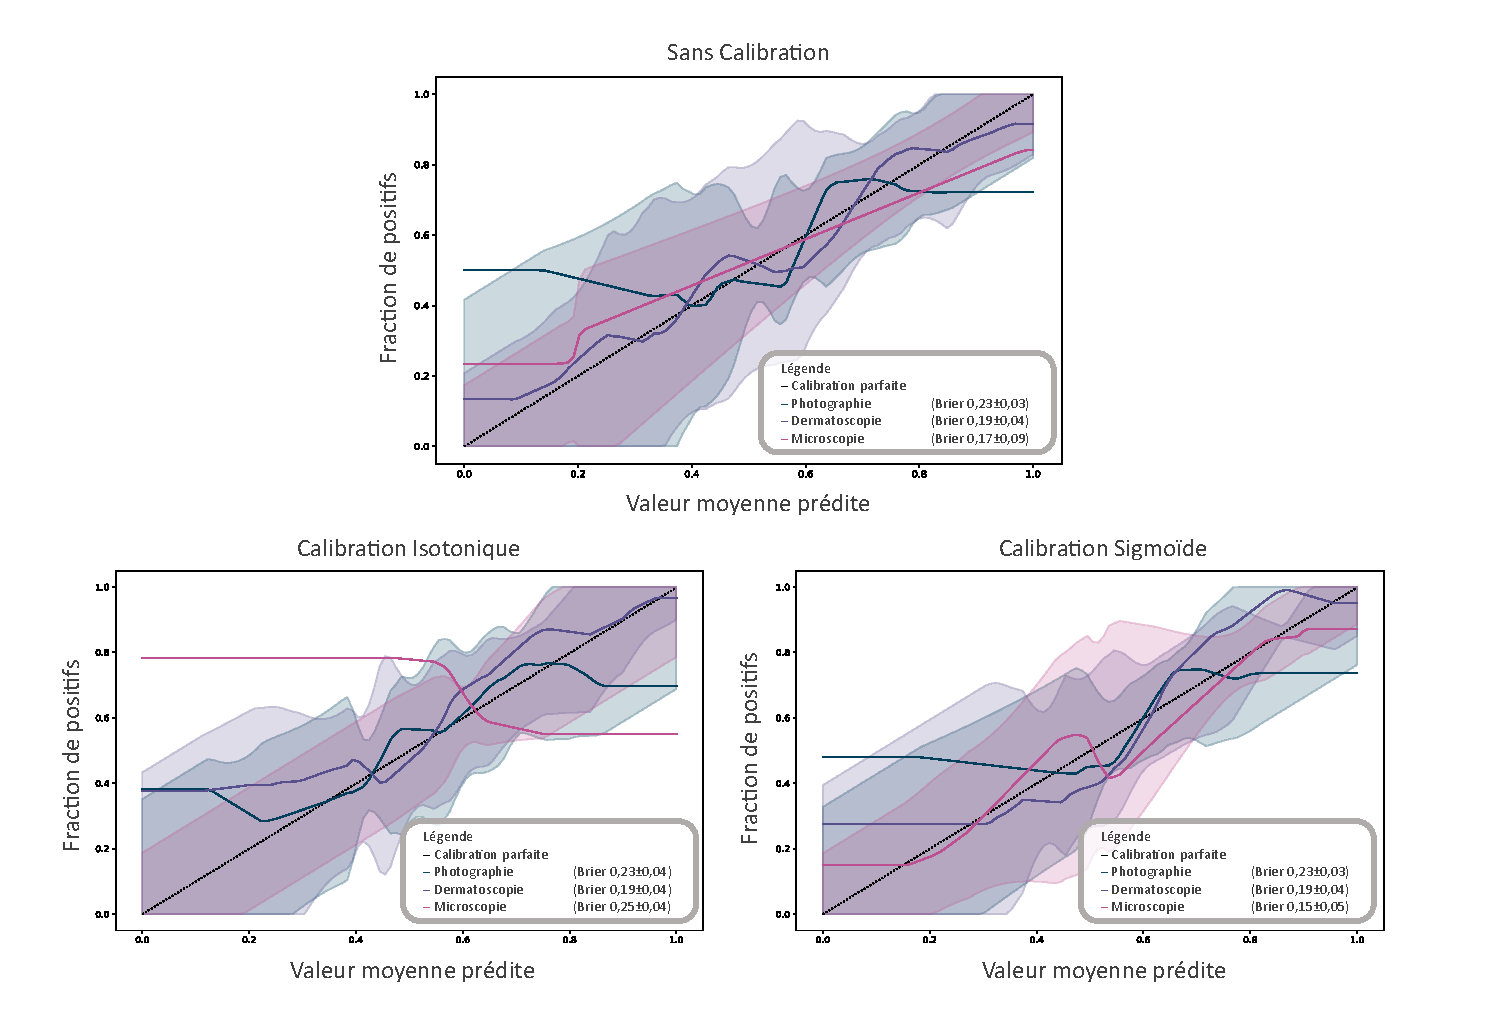
\includegraphics[width=0.8\linewidth]{contents/chapter_8/resources/results_calibration_sequential.pdf}
    \caption{Courbes de calibration et scores de Brier obtenus pour le processus multimodal sans mémoire. L'écart-type calculé sur les différents lots figure en opaque pour les courbes. En haut, le processus multimodal sans calibration~;~À gauche, le processus multimodal avec calibration Isotonique~;~À droite, le processus multimodal avec calibration Sigmoïde.}
    \label{fig:results_calibration_sequential}
\end{figure}
\end{landscape}

\begin{landscape}
\begin{figure}[H]
    \centering
    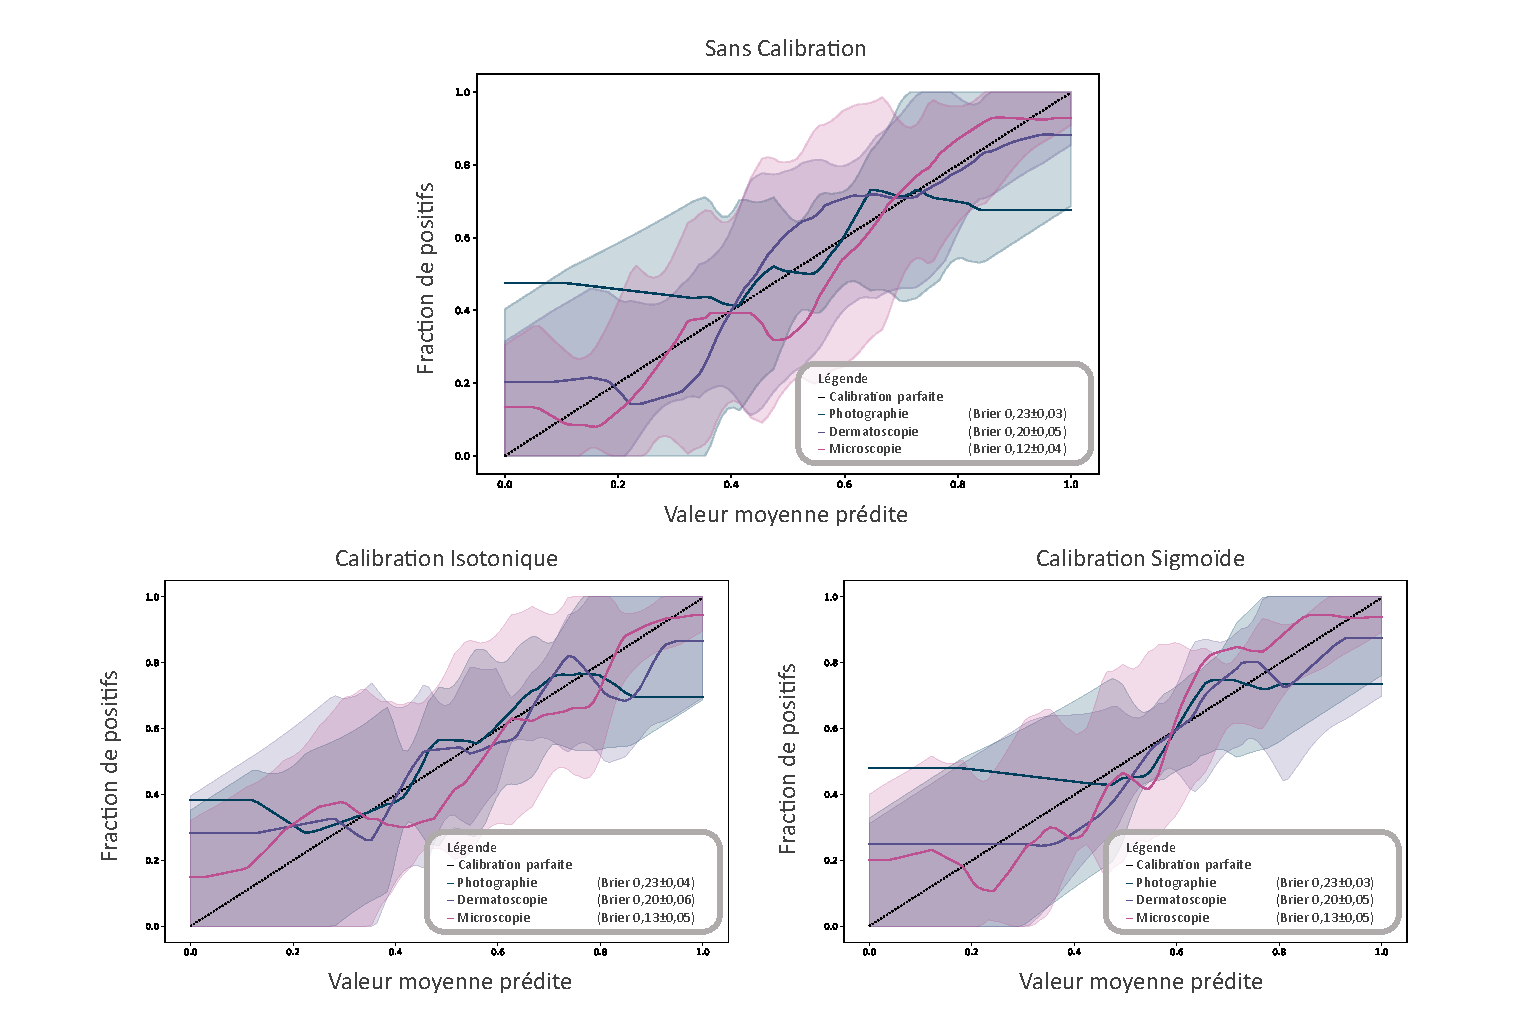
\includegraphics[width=0.8\linewidth]{contents/chapter_8/resources/results_calibration_cumulative.pdf}
    \caption{Courbes de calibration et scores de Brier obtenus pour le processus multimodal avec mémoire. L'écart-type calculé sur les différents lots figure en opaque pour les courbes. En haut, le processus multimodal sans calibration~;~À gauche, le processus multimodal avec calibration Isotonique~;~À droite, le processus multimodal avec calibration Sigmoïde.}
    \label{fig:results_calibration_cumulative}
\end{figure}
\end{landscape}

Pour finir, les résultats de prise en charge sont l'aboutissement de ce chapitre dont la finalité est de permettre une meilleure répartition des cas cliniques. D'une part, en évitant la réalisation d'examens supplémentaires non nécessaires et d'autres part, afin d'éviter une surcharge des services de dermatologie. Pour cela, à partir des processus multimodaux proposés ayant recueilli le meilleur \fscore{} lors du premier et second paragraphe, divers graphiques sont générés automatiquement pour simuler cette prise en charge à partir des seuils déterminés. Dans un premier temps par le principe du \textbf{processus sans mémoire}, la photographie clinique permet de prendre en charge une lésion déterminée comme bénigne par un seuil unique de confiance à 0,93~;~la dermatoscopie permet de prendre en charge six lésions déterminées comme bénignes et 60 lésions déterminées comme malignes par un seuil unique de confiance de 0,80~;~la microscopie confocale permet de prendre en charge 64 lésions déterminées comme bénignes et 83 lésions déterminées comme malignes par un seuil unique de confiance de 0,95. Par ce processus, 18 lésions malignes sont considérées à tort comme bénignes représentées en vert clair et, 23 lésions bénignes sont considérées à tort comme malignes en rouge clair. Dans un second temps par le principe du \textbf{processus avec mémoire}, la photographie clinique permet de prendre en charge trois lésions déterminées comme bénignes par un seuil de confiance à 0,95 et quatre lésions déterminées comme malignes par un seuil de confiance à 0,93~;~la dermatoscopie permet de prendre en charge 18 lésions déterminées comme bénignes par un seuil de confiance à 0,66 et trois lésions déterminées comme malignes par un seuil de confiance de 0,97~;~la microscopie confocale permet de prendre en charge 53 lésions déterminées comme bénignes par un seuil de confiance de 1,00 et 141 lésions déterminées comme malignes par un seuil de confiance de 0,49. Par ce processus, 17 lésions malignes sont considérées à tort comme bénignes représentées en vert clair et, 27 lésions bénignes sont considérées à tort comme malignes en rouge clair. Ces résultats de prise en charge des lésions à l'aide d'un processus séquentiel multimodal sont observables sur la \Cref{fig:results_lesions_management}.\par

\begin{figure}[H]
    \centering
    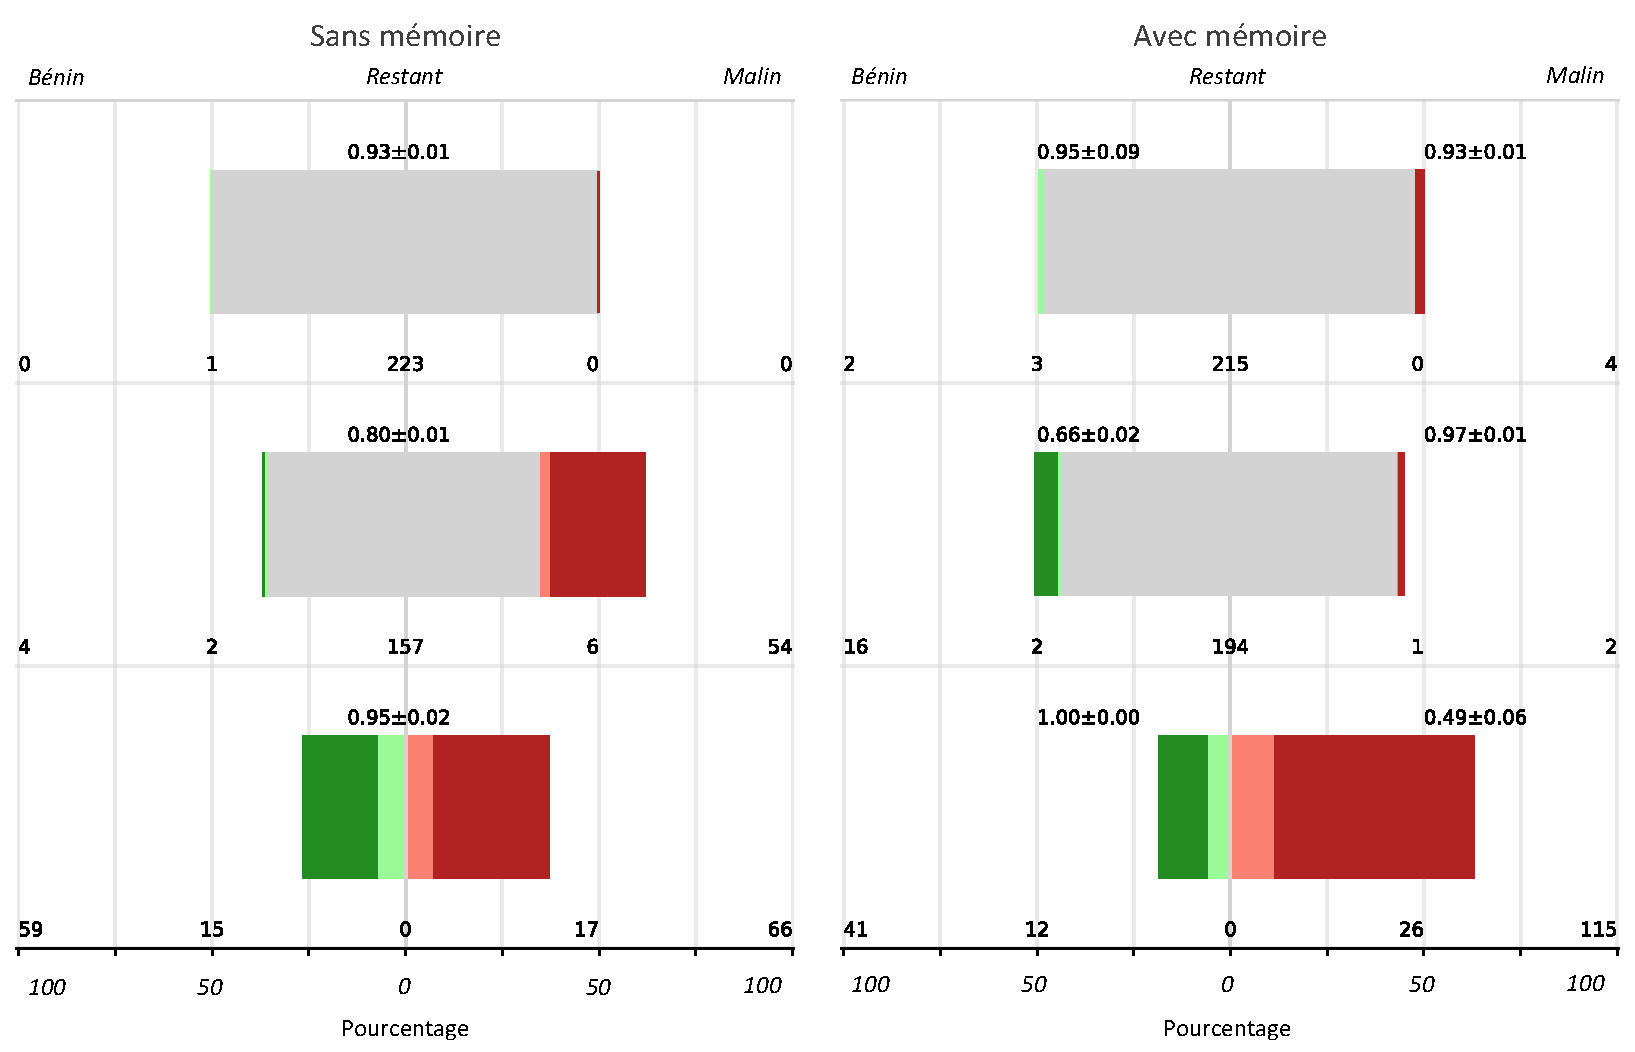
\includegraphics[width=0.9\linewidth]{contents/chapter_8/resources/results_lesions_management.pdf}
    \caption{Résultats de la prise en charge des lésions dans un processus séquentiel multimodal. À gauche, selon un processus sans mémoire~;~À droite, selon un processus avec mémoire. De gauche à droite, les cas bénin correctement classifiés sont représentés en vert foncé~;~les cas bénin incorrectement classifiés sont représentés en vert clair~;~les cas malin incorrectement classifiés sont représentés en rouge clair~;~les cas malin correctement classifiés sont représentés en rouge foncé.}
    \label{fig:results_lesions_management}
\end{figure}\par

\section{Discussion}
Ainsi, différentes propositions de méthodes sont réalisées dans ce chapitre dédié à la prise en charge de lésions de la peau par multimodalité. Lors de la \Cref{sec:modality_diagnosis} consacrée aux méthodes de diagnostic des modalités, le choix s'est porté sur un processus uniforme à l'ensemble des modalités mise à disposition de ce travail. La pertinence de ces modalités s'est avéré suivre le processus de prise en charge clinique, avec un \fscore{} dont la valeur s'accroît pour chaque évaluation réalisée selon ce processus. Néanmoins, la stabilité de prédiction semble suivre une démarche opposée, avec une valeur de 0,08 pour la photographie clinique qui atteint 0,12 avec la \gls{mcr} par les résultats de l'évaluation pondérée. L'un des facteurs à prendre en compte \textbf{est celui de la quantité de données}, de l'ordre de la centaine pour la photographie clinique ainsi que la dermatoscopie, et de l'ordre du millier pour les données de la modalité \gls{mcr}.\par

Cette pertinence croissante dans la qualité du diagnostic donne lieu à un processus global de prise en charge des lésions dans lequel \textbf{une modalité de rang supérieur est sollicitée tant que la confiance dans un diagnostic est jugée insuffisante}. Sur ce principe, deux processus types sont définis pour répondre à cette tâche, le premier \textit{sans mémoire} et le second \textit{avec mémoire}. Dans un premier temps, \textbf{aucune différence notable n'est à reporter en termes de \fscore{} entre la proposition à seuil unique et à seuils multiples}, avec initialement un risque de sur-apprentissage plus grand pour cette seconde proposition qui ne s'est pas manifesté lors de ces expérimentations. Dans un second temps, plusieurs hypothèses ont été formulées pour permettre la recherche des seuils de confiance. La première de ces hypothèses consiste à rechercher les seuils de confiance optimaux soit par amélioration, c'est-à-dire en partant de la modalité la moins précise, soit par dégradation des résultats, c'est à dire en partant de la modalité la plus précise. Les mesures de \fscore{} obtenues \textbf{par dégradation des résultats sont ainsi sensiblement supérieures à celles obtenue par amélioration des résultats}. La seconde de ces hypothèses consiste à déterminer le sens de recherche des seuils de confiance, aboutissant à déterminer les seuils de manière la plus \textit{restrictive} (seuil haut) ou la plus \textit{laxiste} (seuil bas). Ainsi, cette seconde hypothèse \textbf{n'amène aucune différence dans le cadre du processus sans mémoire, tandis que sont influence peut être remarquée dans le processus avec mémoire}.\par

Afin d'apporter une plus grande signification aux scores issus de la classification et dans le but d'améliorer les scores précédents, le principe de la calibration de modèles est également exploré dans ce chapitre. Sur les nombreuses méthodes de calibration existantes, seules les méthodes de calibrations isotonique et sigmoïde, sont appliquées aux modèles de prédiction composants les deux processus de prise en charge proposées. Ainsi, quel que soit le processus considéré de prise en charge des lésions, \textbf{l'utilisation de ces méthodes de calibration à le plus souvent dégradé la qualité des résultats précédemment obtenus}. Pour la méthode de calibration sigmoïde, l'une des explications possibles est l'inadéquation entre la courbe de calibration initiale de ces modèles et la fonction de correction sigmoïde, visible en \Cref{fig:results_calibration_sequential} et \Cref{fig:results_calibration_cumulative}. Pour les deux méthodes de calibration, le faible nombre d'éléments mis à disposition de l'entraînement de ces méthodes suscite un doute non négligeable et particulièrement pour la calibration isotonique plus enclin au sur-apprentissage. Ces aspects de calibration sont à améliorer dans de futurs travaux menés sur cette thématique, dans le but d'améliorer la correspondance entre les scores et les probabilités des modèles de classification employés, et de réduire par la même occasion la variabilité des prédictions.\par
\clearpage

En définitive, bien que le processus avec mémoire soit supérieure au processus sans mémoire, la différence entre ces deux modes de prise en charge n'est pas notable, avec respectivement un \fscore{} pondéré de 0,82 et de 0,80. Néanmoins, il est important de souligner que ce ne processus n'augmente pas la qualité des prédictions réalisées. En effet, l'une des hypothèses formulée initialement était qu'une restriction des cas les plus confiant pouvait permettre d'augmenter la qualité du diagnostic final, ce que ce travail ne parvient pas à accomplir. Ainsi, dans leur état actuel ces processus de prise en charge multimodaux peuvent être davantage perçu comme un compromis entre l'exactitude des détections et la répartition des cas cliniques tout au long du processus. Comparativement, le processus sans mémoire retenu gère mieux la répartition des lésions tout au long des modalités que celui avec mémoire, mais avec un compromis sur le \fscore{} dont la valeur pondérée est de 0,80 contre une valeur de 0,82.\par

